\documentclass[conference]{IEEEtran}
\usepackage{graphicx}
\usepackage{tikz}
 
\usepackage[colorlinks = true, citecolor = blue]{hyperref}

% math lib
\usepackage{amsmath}
\usepackage{mathrsfs}

% operators
\DeclareMathOperator*{\argmax}{arg\,max}
\DeclareMathOperator*{\argmin}{arg\,min}
\newcommand\ceiling[1]{\left\lceil #1 \right\rceil}

% empty set
\usepackage{amssymb}
\let\emptyset=\varnothing

% algorithms
\usepackage{algorithm}
\usepackage{algorithmic}
\renewcommand{\algorithmicrequire}{\textbf{Input:}}
\renewcommand{\algorithmicensure}{\textbf{Output:}}

\begin{document}
% --------------------------------------------
% --------------Change HERE! -----------------
% --------------------------------------------
\def\authorone{Mrunal Zambre}
\def\authortwo{Anahita Dinesh}
\def\groupid{7}
% --------------------------------------------
\title{CS258 Final Report: The RSA Problem}
\author{
    \IEEEauthorblockN{\authorone\ and \authortwo}
    \IEEEauthorblockA{
        Group \groupid
    }    
}

\maketitle
\IEEEpeerreviewmaketitle


\section{Methods: RL-based Routing}


\subsection{RL Algorithms}
In our project, we have employed two prominent reinforcement learning algorithms, Proximal Policy Optimization (PPO) and Importance Weighted Actor-Learner Architectures (IMPALA), to tackle the problem of routing and spectrum allocation. Both algorithms are well-regarded for their balance between performance and computational efficiency.
% List RL algorithms and give a brief explanation of each
\subsubsection{PPO}
Proximal Policy Optimization (PPO) \cite{DBLP:journals/corr/SchulmanWDRK17} is currently regarded as a leading algorithm in reinforcement learning. PPO is a model-free, policy optimization gradient-based algorithm designed to learn a policy that maximizes cumulative rewards based on the training experience. It consists of an actor, which generates a probability distribution for the next action given the state at time t, and a critic, which estimates the expected cumulative reward from that state. Both the actor and critic use the state as input, allowing them to share a backbone architecture for extracting high-level features. PPO works by making the policy more likely to select actions with a high "advantage", meaning those actions that yield a significantly higher cumulative reward than predicted by the critic. An architecture provided by rllib documentation is depicted in Figure \ref{fig:your_label_ppo}
\begin{figure}[h!]
    \centering
    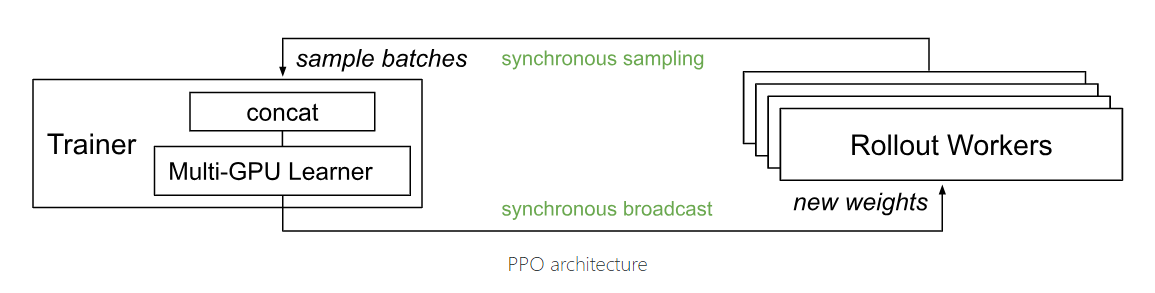
\includegraphics[width=\columnwidth]{images/ppo.png}
    \caption{PPO Architecture from rllib documentation}
    \label{fig:your_label_ppo}
\end{figure}

\subsubsection{IMPALA}
IMPALA\cite{DBLP:journals/corr/abs-1802-01561} is an off-policy actor-critic framework that separates the acting process from the learning process and learns from experience trajectories using V-trace. IMPALA actors send trajectories of experience (sequences of states, actions, and rewards) to a centralized learner. The learner, having access to full trajectories, uses a GPU to update mini-batches of these trajectories while parallelizing time-independent operations for efficiency. This decoupled architecture allows for very high throughput. IMPALA is a model-free and off-policy reinforcement learning algorithm that supports both discrete and continuous action spaces. As an actor-critic algorithm, IMPALA optimizes both the actor network and the critic (value) network. It can leverage old off-policy data with appropriate corrections to stabilize learning. IMPALA's architecture decouples data collection from learning, with collectors not computing value or advantage. The loss functions used in IMPALA are similar to those in PPO, and other actor-critic models. An architecture provided by rllib documentation is depicted in Figure \ref{fig:your_label_impala}
\begin{figure}[h!]
    \centering
    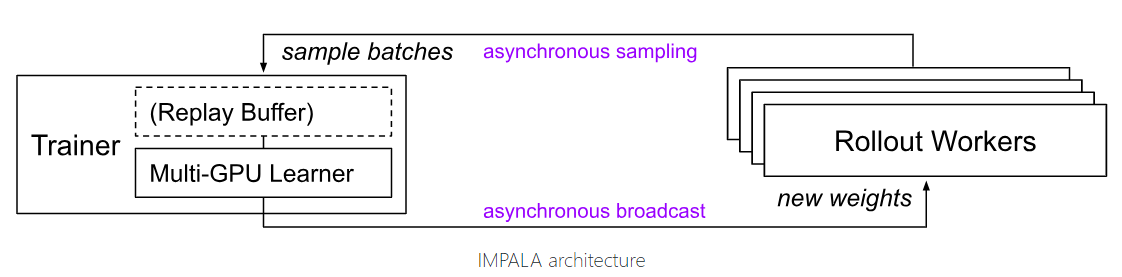
\includegraphics[width=\columnwidth]{images/impala.png}
    \caption{IMPALA Architecture from rllib documentation}
    \label{fig:your_label_impala}
\end{figure}

\subsection{State Space}
% Explain state/action/reward
% Make sure you provide enough information to reconstruct results
% Check https://gymnasium.farama.org/environments/box2d/lunar_lander/ for some examples

The state space (observation space) in a reinforcement learning environment defines all the possible states in which the agent can exist. In our network simulation environment, the observation space is represented by a dictionary with two main components:

1. \textbf{Edge Capacities}: This is represented as a 15x10 matrix, where each entry corresponds to the current holding time left for a request on a given edge in the network. The value -1 indicates no request is currently using that slot, and values between 0 and 20 represent the remaining holding times of active requests. The matrix dimensionality (15 edges, each with up to 10 concurrent requests) encapsulates the simultaneous capacity constraints of the network.

2. \textbf{Request}: This is a nested dictionary containing three elements:

1. Source (src): A single integer representing the source node of a request, ranging from 0 to 12.

2. Destination (dest): A single integer that specifies the destination node, similarly ranging from 0 to 12.

3. Holding Time (ht): The time that the request needs to hold the resource, ranging from 10 to 20 units.

\subsection{Action Space}

The action space defines all the possible actions that the agent can take in any given state. In this environment, the action space consists of discrete choices corresponding to possible paths a request can take through the network, plus an additional action to block a request if no viable path is available.

\textbf{Case 1:} In this scenario, the source and destination nodes were predetermined, allowing us to identify exactly seven viable paths for routing. In addition to these paths, we included an option to block the request if necessary. Therefore, the action space was defined as a set of eight discrete actions, numbered from 0 to 7, where actions 0 through 6 correspond to the seven paths, and action 7 is reserved for blocking the request.

\textbf{Case 2:} Here, the source and destination nodes were chosen randomly, which introduced variability in the number of feasible paths between node pairs. However, we found that every source-destination pair had at most eight possible paths. To accommodate this, we defined the action space to include eight paths plus an additional action for blocking, resulting in a total of nine discrete actions, numbered from 0 to 8. This setup ensures that the agent always has a consistent set of choices regardless of the specific nodes involved. In instances where the agent chose a path that did not exist for the specified source-destination pair, we defaulted to blocking the request. 

\subsection{Reward Function}
The reward function is designed to guide the agent's learning process towards the most effective strategies for managing network traffic:

\textbf{Case 1:}
\begin{itemize}
\item Positive Reward: The agent receives a positive reward when it selects an action that the network can accommodate. This reward is determined by the average utilization of all edges on the chosen path. Specifically, the reward is calculated as the total capacity of an edge minus its average utilization.

\item Negative Reward: A negative reward of -10 is given if the agent either blocks the request or selects a path that lacks the capacity to handle the request.
\end{itemize}

\textbf{Case 2:}
\begin{itemize}
\item Positive Reward: In this scenario, we calculate the reward based on the total network utilization, rather than just the utilization of the chosen path. This involves calculating the network's utilization before and after the request is accommodated, with the reward corresponding to the change in utilization.

\item Negative Reward: If the agent opts to block a request, it incurs a negative reward of -4. If the agent selects a non-existent path for the given source-destination pair, or if it chooses a path that currently lacks capacity, a higher penalty of -8 is applied to penalize the wrong action more severely.
\end{itemize}


\section{Method: Spectrum Allocation}
% Explain your heuristic
% If you have multiple, you can make subsections 

% If you borrow some ideas from papers, cite them with bibtex (e.g. \cite{8509143})

To perform spectrum allocation, we implemented a straightforward heuristic centered on the smallest index allocation, which varied between the two scenarios.

\textbf{Case 1}: 
\begin{itemize}
    \item Process: When the agent selects a path, the allocation process begins by identifying the smallest available capacity index on the first edge of the chosen path. Given that all requests have the same source-destination pair, it was not necessary to verify availability across the same index for all edges, as every request originates from the same initial edge. Therefore, the first smallest available index identified was always suitable for accommodating the current request.
    \item Update and Reward: We then update the observation of the edge states with the request’s holding time for each edge along the path at this smallest available index. If no capacity is available on the first edge, the request is blocked, resulting in a negative reward for the agent.
\end{itemize}


\textbf{Case 2}: 
\begin{itemize}
    \item Process: With varying source-destination pairs in this scenario, it was necessary to ensure that the same index is available across all edges in the chosen path, as the request cannot be split across different indices. We start by obtaining a sorted list of all available indices for the first edge. We then check each index to find the smallest one available across all edges in the path.
    \item Update and Reward: Once the smallest consistent index is found, we update the observation of edge states to reflect the holding times across all edges for that index. If no consistent index is available, the request is blocked, and a negative reward is issued to the agent.
\end{itemize}


\section{Results}
\subsection{Learning Curve}
% Insert figures
% Explain the results

In our project, we utilized the Proximal Policy Optimization (PPO) and IMPALA algorithms across both scenarios. 

\textbf{1. PPO} 

Figure \ref{fig:lc_c1_ppo} illustrates the learning curve generated by Tensorboard, represented as reward versus episode number, for Case 1 using the PPO algorithm. For training this model, we set a learning rate of 0.003 and a gamma of 0.999, optimizing our algorithm's ability to balance immediate and future rewards effectively.
The learning curve for Case 1 shows that the PPO algorithm (black curve) has a fluctuating yet overall increasing trend in average reward over episodes, indicating gradual learning and adaptation, whereas the baseline (blue curve), with a zero learning rate, remains relatively flat and consistently lower, demonstrating no learning progress.

\begin{figure}[htp]
    \centering
    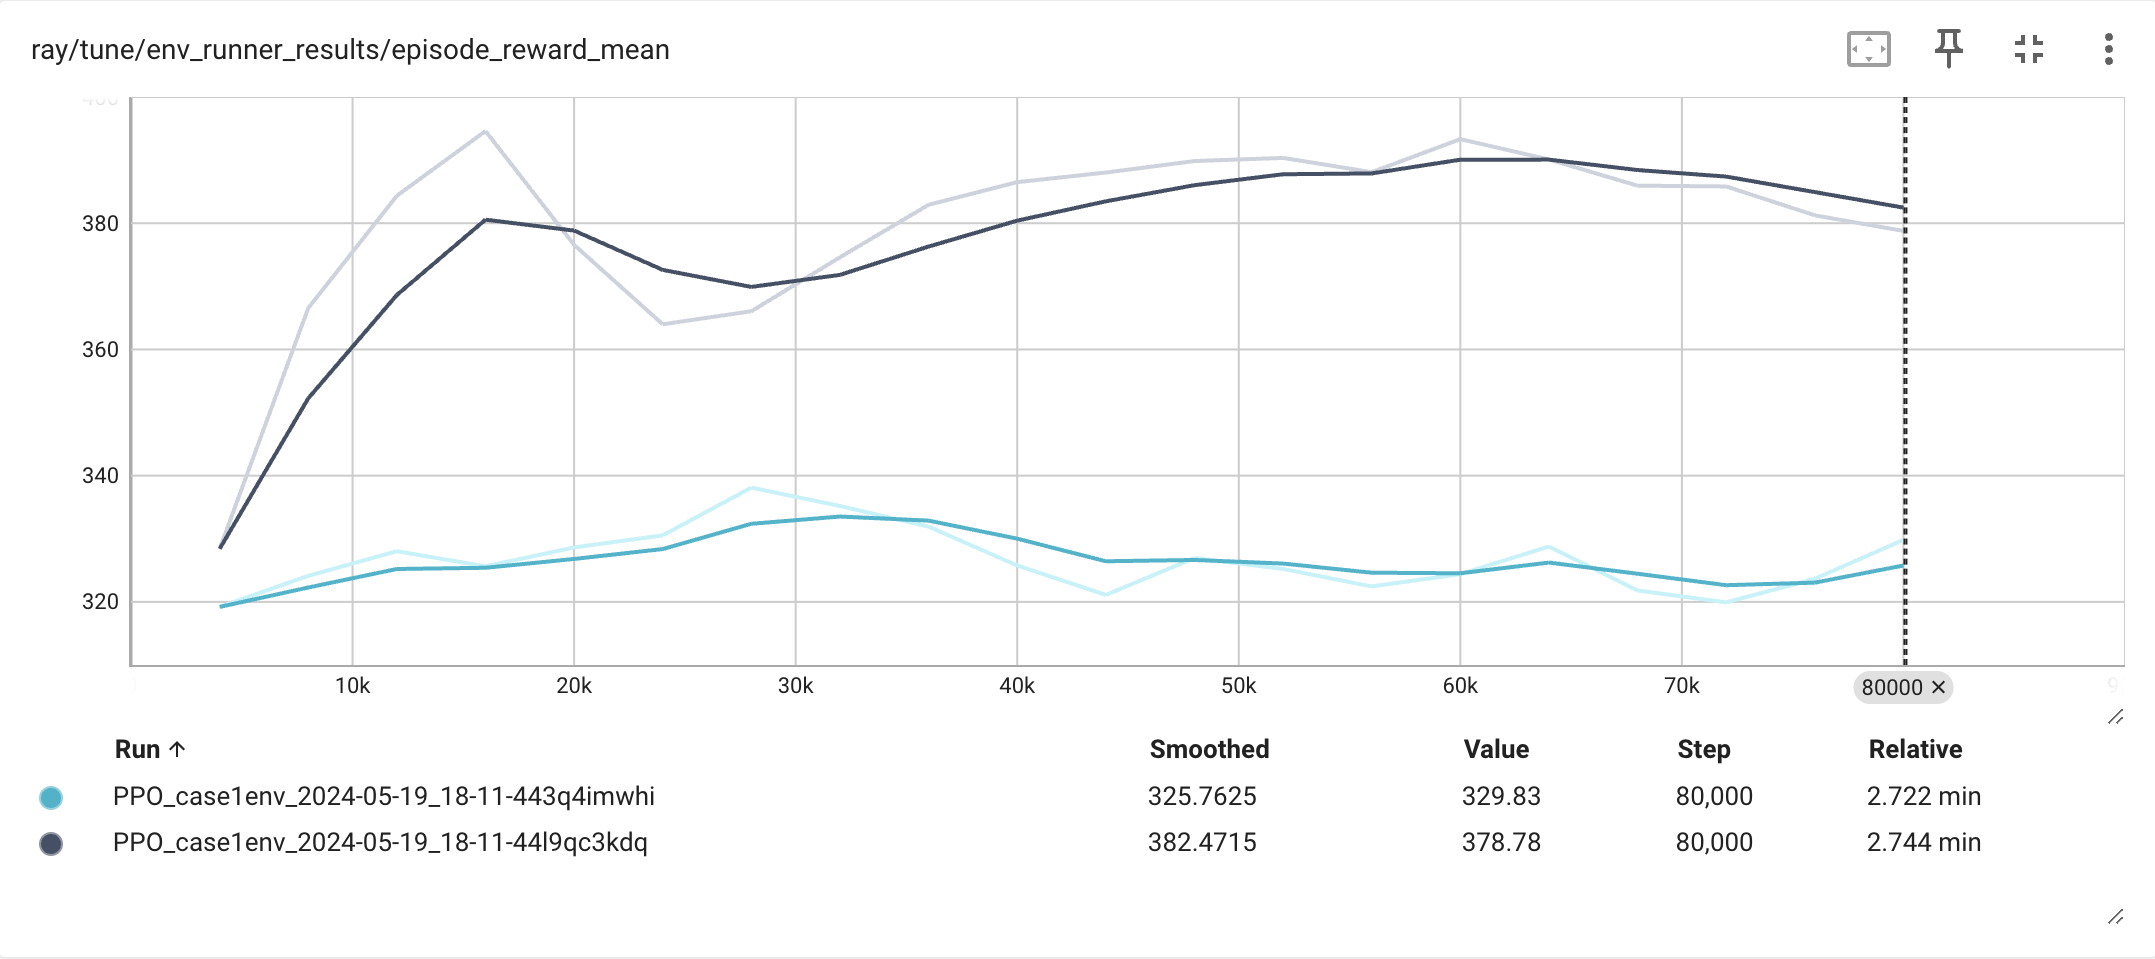
\includegraphics[width=8cm]{images/LC_case1_PPO.png}
    \caption{Learning curve for Case 1 with PPO (reward vs episode)}
    \label{fig:lc_c1_ppo}
\end{figure}

Figure \ref{fig:lc_c2_ppo} shows the learning curve for Case 2 using the PPO algorithm.For this specific scenario, we opted for a higher learning rate of 0.008, while maintaining the same gamma value of 0.999, to achieve a more rapid adaptation to the more varied conditions in Case 2. The learning curve for Case 2 shows that the PPO algorithm (black curve) exhibits a significant upward trend in average reward over episodes, suggesting effective learning and optimization. In contrast, the baseline (blue curve), with no learning capability due to a zero learning rate, remains consistently lower and flat, indicating no improvement over time. 


\begin{figure}[htp]
    \centering
    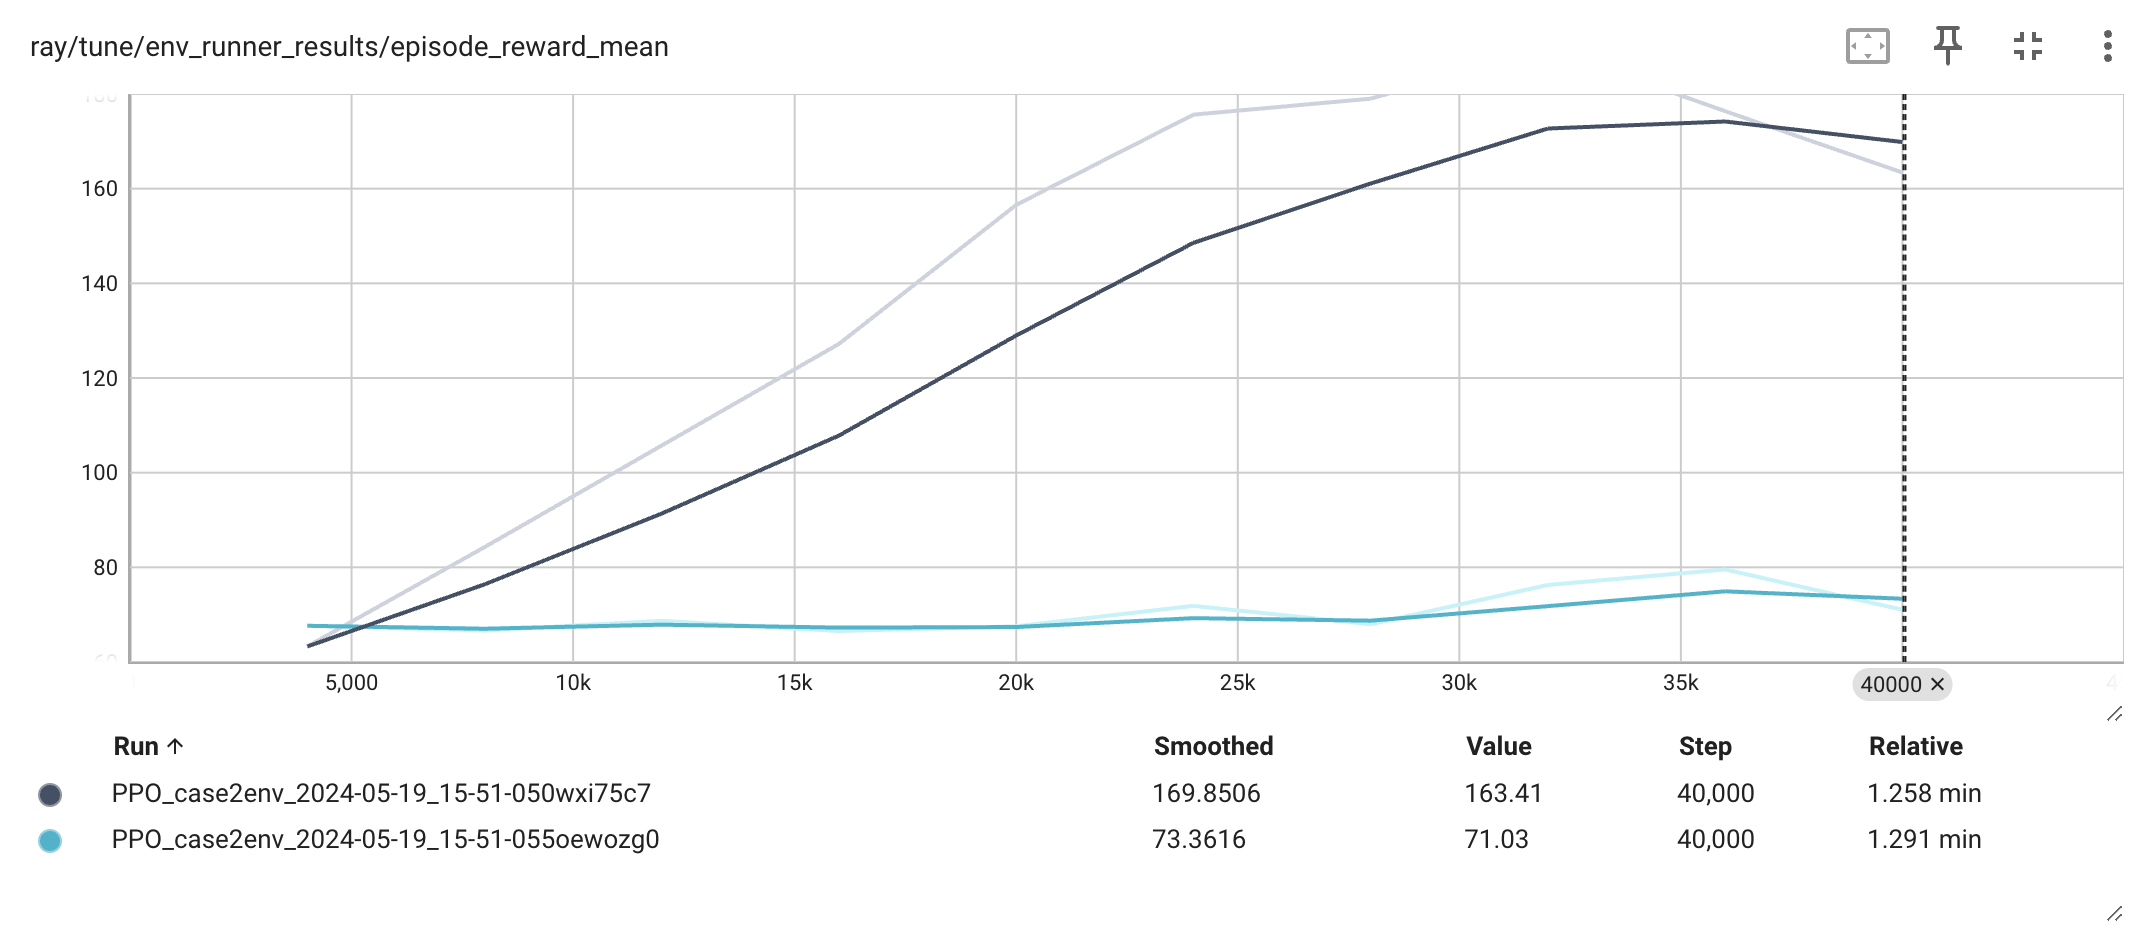
\includegraphics[width=8cm]{images/LC_case2_PPO.png}
    \caption{Learning curve for Case 2 with PPO (reward vs episode)}
    \label{fig:lc_c2_ppo}
\end{figure}


\textbf{2. IMPALA}

Figure \ref{fig:impala_case1} shows that shows the learning curve for Case 1 using the IMPALA algorithm. Learning rate 0.0003 and gamma value of 0.999 was used in training. The light blue curve represents the baseline run with a learning rate of zero. As expected, this curve shows little to no improvement over time, maintaining relatively low and stable mean episode rewards. The black curve represents the run with active learning using the IMPALA algorithm. Initially, the mean episode reward increases, indicating that the algorithm is learning and improving its policy. The rewards rise sharply up, reaching a high reward mean of around 380. After reaching the peak, the black curve begins to decline, with the mean episode reward dropping as training continues. This could suggest potential over-fitting and a need for further hyper parameter tuning.
\begin{figure}[htp]
    \centering
    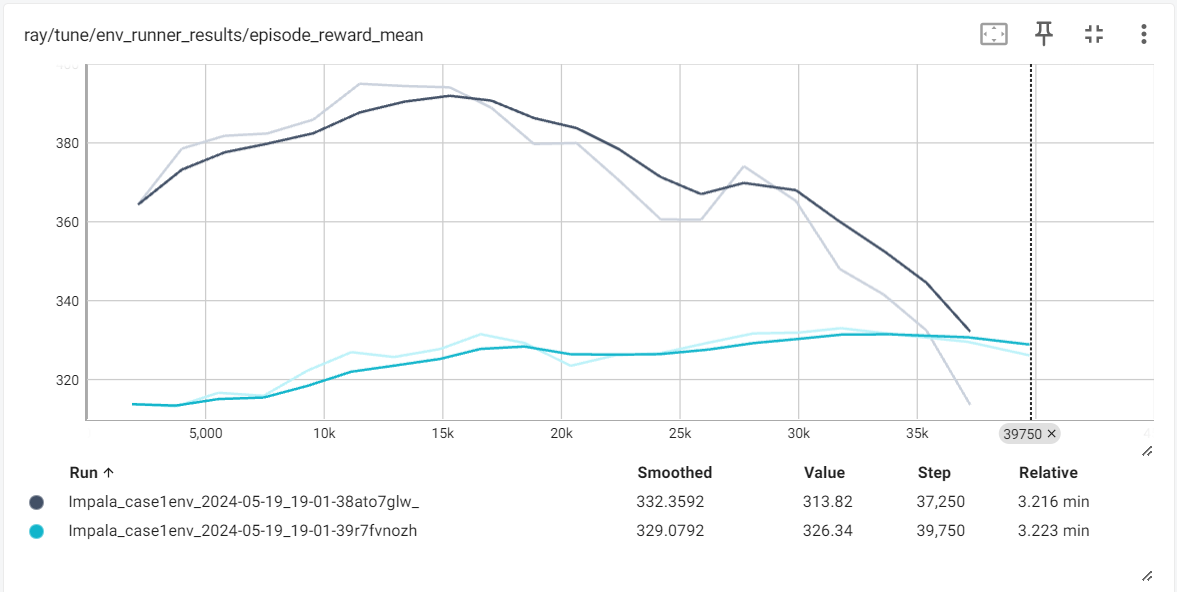
\includegraphics[width=\columnwidth]{images/LC_case1_IMPALA.png}
    \caption{Learning curve for Case 1 with IMPALA (reward vs episode)}
    \label{fig:impala_case1}
\end{figure}

Figure \ref{fig:impala_case2} shows that shows the learning curve for Case 2 using the IMPALA algorithm. For this scenario, we opted for a learning rate of 0.003 and a gamma value of 0.999. The steady increase and higher values in the mean episode reward for the black curve indicate successful learning and adaptation by the IMPALA algorithm. In contrast, the baseline (blue curve), did not learn at all due to its assigned learning rate of 0.0, and thus, remains consistently lower and flat, indicating no improvement over time.

\begin{figure}[htp]
    \centering
    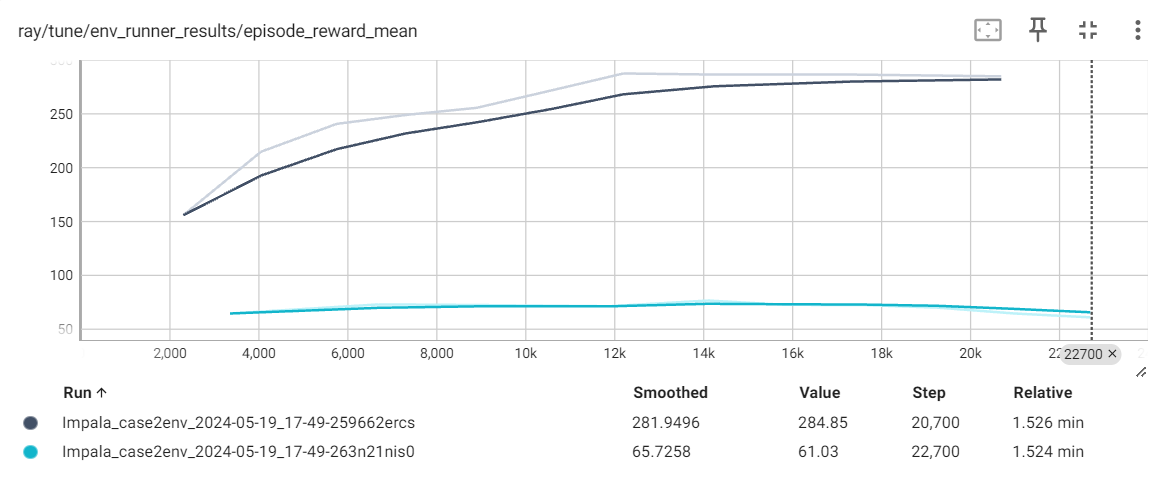
\includegraphics[width=\columnwidth]{images/LC_case2_IMPALA.png}
    \caption{Learning curve for Case 2 with IMPALA (reward vs episode)}
    \label{fig:impala_case2}
\end{figure}

\subsection{Utilization (The Objective)}

In this project, our goal is to maximize the utilization of optical resources throughout the network. The network-wide utilization is defined as the average utility of all edges, as described in figure \ref{fig:equation_obj}.

\begin{figure}[htp]
    \centering
    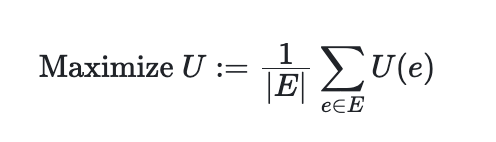
\includegraphics[scale=0.6]{images/equation_objective.png}
    \caption{Objective Function}
    \label{fig:equation_obj}
\end{figure}

To achieve this, we tracked the utilization across all network edges for each request. We then computed the average utilization for each link, enabling us to determine the overall average network-wide utilization.

\textbf{1. PPO}

For Case 1 utilizing the PPO algorithm, we conducted training over 20 iterations with each iteration comprising 40 episodes, thus accumulating data on average network utilization across a total of 800 episodes. We plotted the graph for this data in Figure \ref{fig:obj_c1_ppo}. Overall, the plot shows a relatively stable trend in network utilization, with minor fluctuations throughout the episodes. The data density and the range suggest that while there are variations in network utilization from episode to episode, the overall system maintains a moderately high level of utilization.

\begin{figure}[htp]
    \centering
    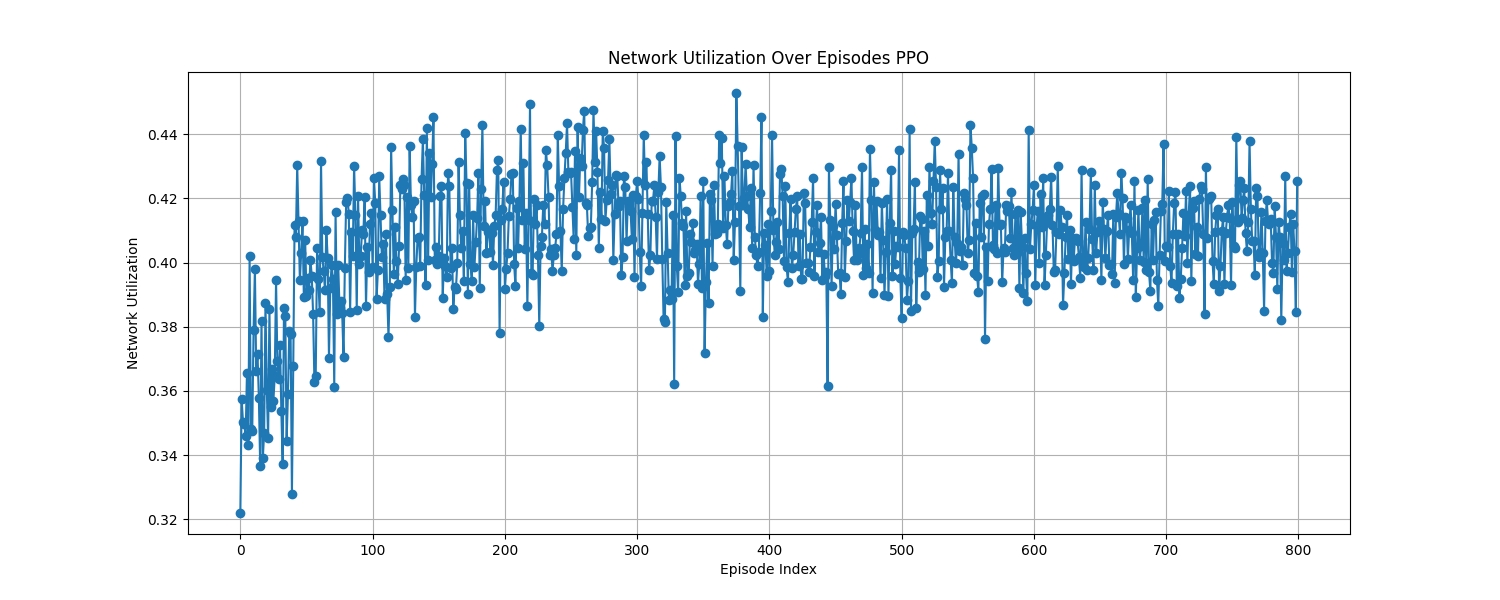
\includegraphics[width=\columnwidth]{images/obj_fn_case1_PPO.png}
    \caption{Increase in Objective Function for Case 1 with PPO}
    \label{fig:obj_c1_ppo}
\end{figure}


Similarly, for Case 2 with the PPO algorithm, the training was conducted over 10 iterations, also with 40 episodes per iteration, resulting in data collection on average network utilization across 400 episodes. We plotted the graph for this data in Figure \ref{fig:obj_c2_ppo}. Compared to the plot for case 1, this one shows more significant fluctuations and generally lower utilization levels. The broader range and more pronounced peaks and troughs indicate a less stable network utilization, which could suggest more variability in the network conditions posed by the scenarios in Case 2.


\begin{figure}[htp]
    \centering
    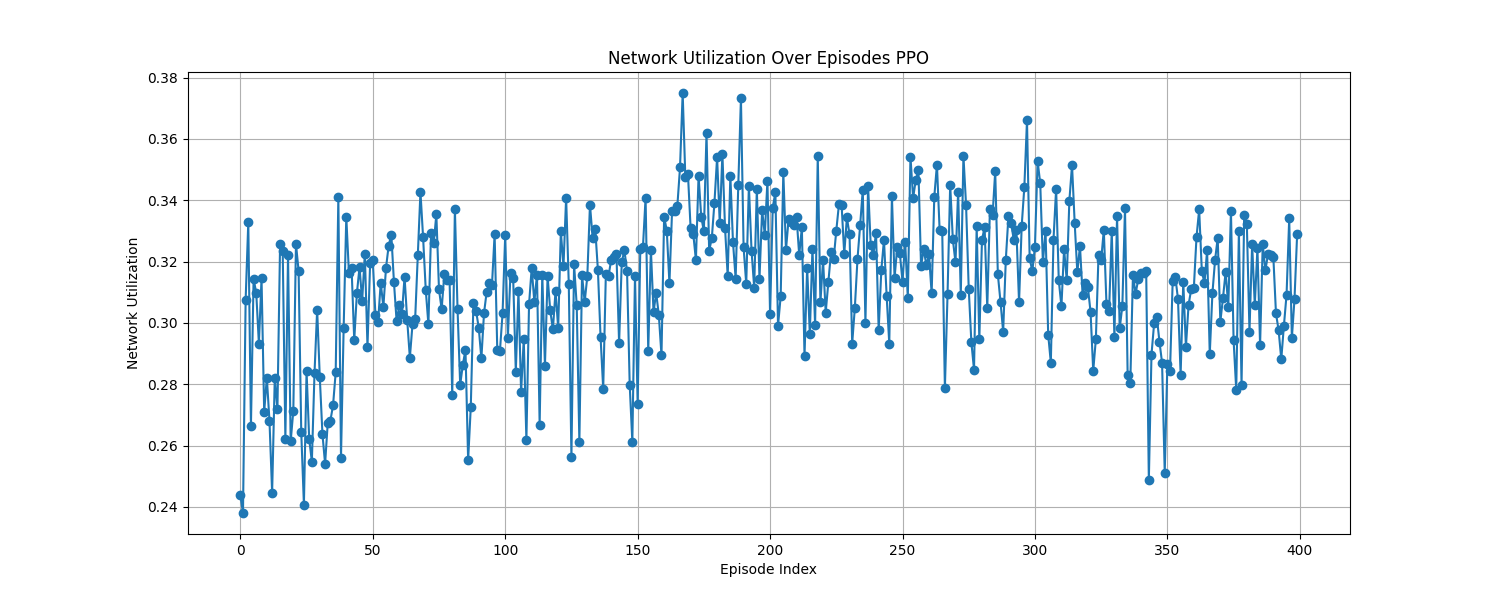
\includegraphics[width=\columnwidth]{images/obj_fn_case2_PPO.png}
    \caption{Increase in Objective Function for Case 2 with PPO}
    \label{fig:obj_c2_ppo}
\end{figure}

\textbf{2. IMPALA}

For Case 1 with the IMPALA algorithm, the training was conducted over 20 iterations, also with 40 episodes per iteration, resulting in data collection on average network utilization across 800 episodes. We plotted the graph for this data in Figure \ref{fig:obj_c1_impala}. The fluctuation in the data points in this graph indicate that the IMPALA algorithm might have been adjusting to certain conditions or exploring different strategies, which temporarily led to lower utilization. The recovery and stabilization suggest that the algorithm adapted and improved its strategies for managing network resources as episodes progressed.

\begin{figure}[htp]
    \centering
    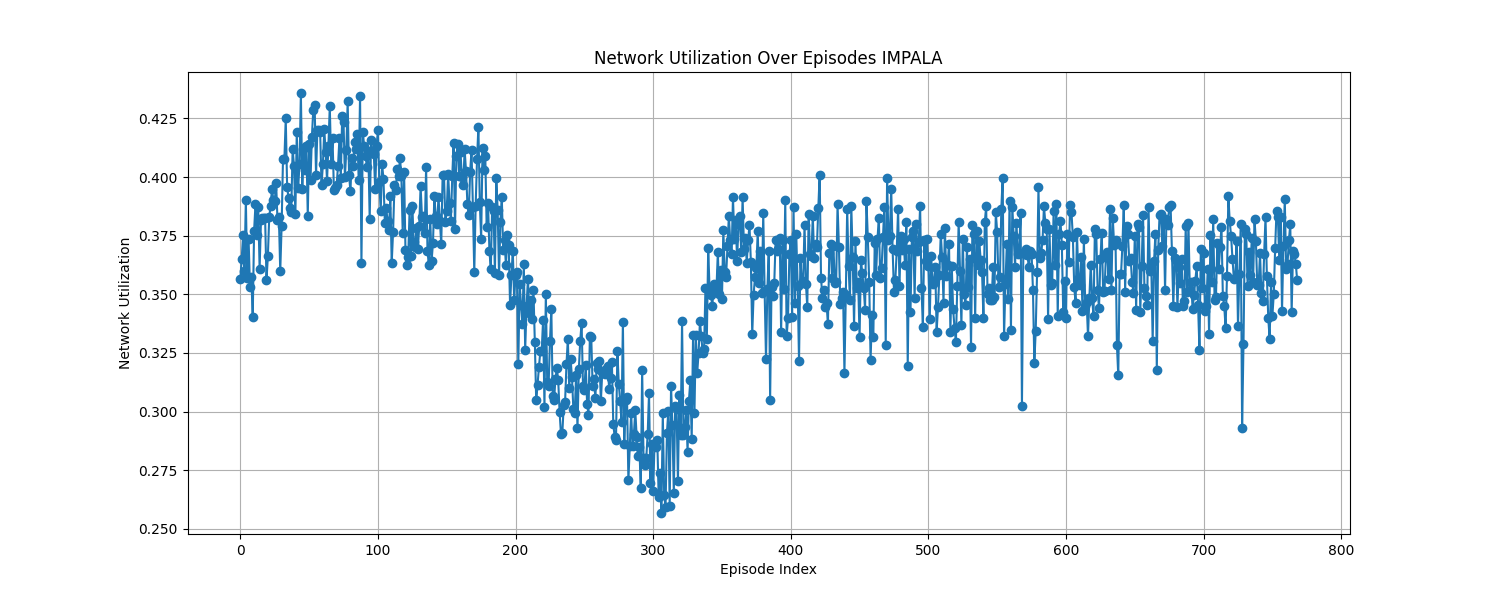
\includegraphics[width=\columnwidth]{images/obj_fn_case1_impala.png}
    \caption{Increase in Objective Function for Case 1 with IMPALA}
    \label{fig:obj_c1_impala}
\end{figure}



For Case 2 with the IMPALA algorithm, the training was conducted over 10 iterations, also with 40 episodes per iteration, resulting in data collection on average network utilization across 400 episodes. We plotted the graph for this data in Figure \ref{fig:obj_c2_impala}. The data points show significant variability across the episodes. This fluctuation suggests that the network conditions or the algorithm's decisions in this case are highly dynamic, with network utilization sometimes dipping considerably before recovering. This behavior indicates that the IMPALA algorithm experiences periods of both high and low efficiency in managing network resources within this more complex scenario 2.

\begin{figure}[htp]
    \centering
    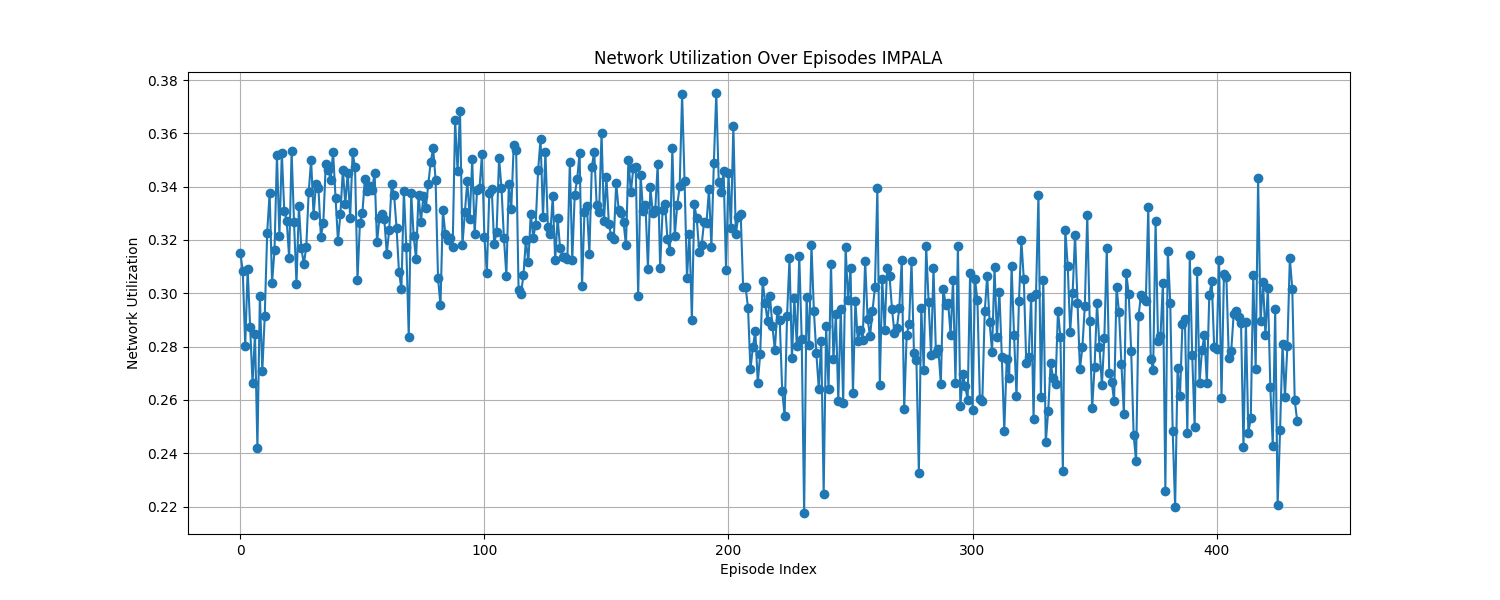
\includegraphics[width=\columnwidth]{images/obj_fn_case2_impala.png}
    \caption{Increase in Objective Function for Case 2 with IMPALA}
    \label{fig:obj_c2_impala}
\end{figure}



\subsection{Comparison}

Lastly, we aimed to compare the performance of the two reinforcement learning algorithms—PPO and IMPALA—with a simple heuristic method that utilizes the shortest path combined with smallest index allocation to manage network resources. To show this comparison, we computed the average network-wide utilization for the heuristic approach as well and integrated these results into a comprehensive graph. 

The graph for comparison between the three methods for Case 1 is presented in Figure \ref{fig:comp_c1}. It reveals that the PPO algorithm (denoted by red curve) generally achieves higher and more stable network utilization compared to IMPALA (denoted by blue curve) with the Simple Heuristic method (denoted by grey curve) demonstrating consistent performance at a lower level. IMPALA exhibits the most variability, indicating a possible sensitivity to episode conditions or a less stable learning process.

\begin{figure}[htp]
    \centering
    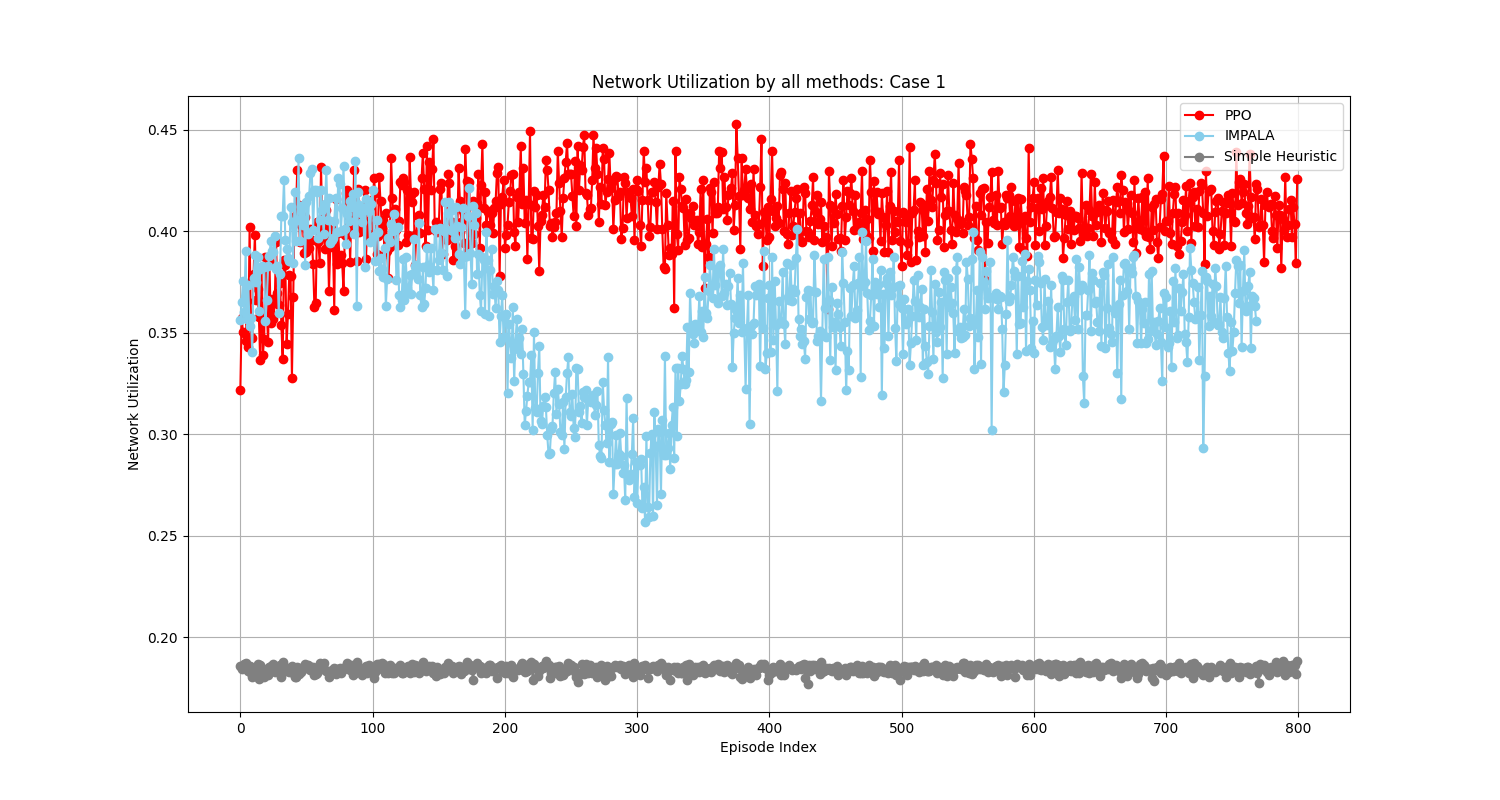
\includegraphics[width=\columnwidth]{images/comparison_case1.png}
    \caption{Comparison between methods for Case 1}
    \label{fig:comp_c1}
\end{figure}

The graph for comparison between the three methods for Case 2 is presented in Figure \ref{fig:comp_c2}. In Case 2, PPO (red) shows better peak performance but with noticeable fluctuations, while IMPALA (blue) continues to display significant variability with both high peaks and deep troughs. The Simple Heuristic (grey) maintains a steady and lower utilization throughout.


\begin{figure}[htp]
    \centering
    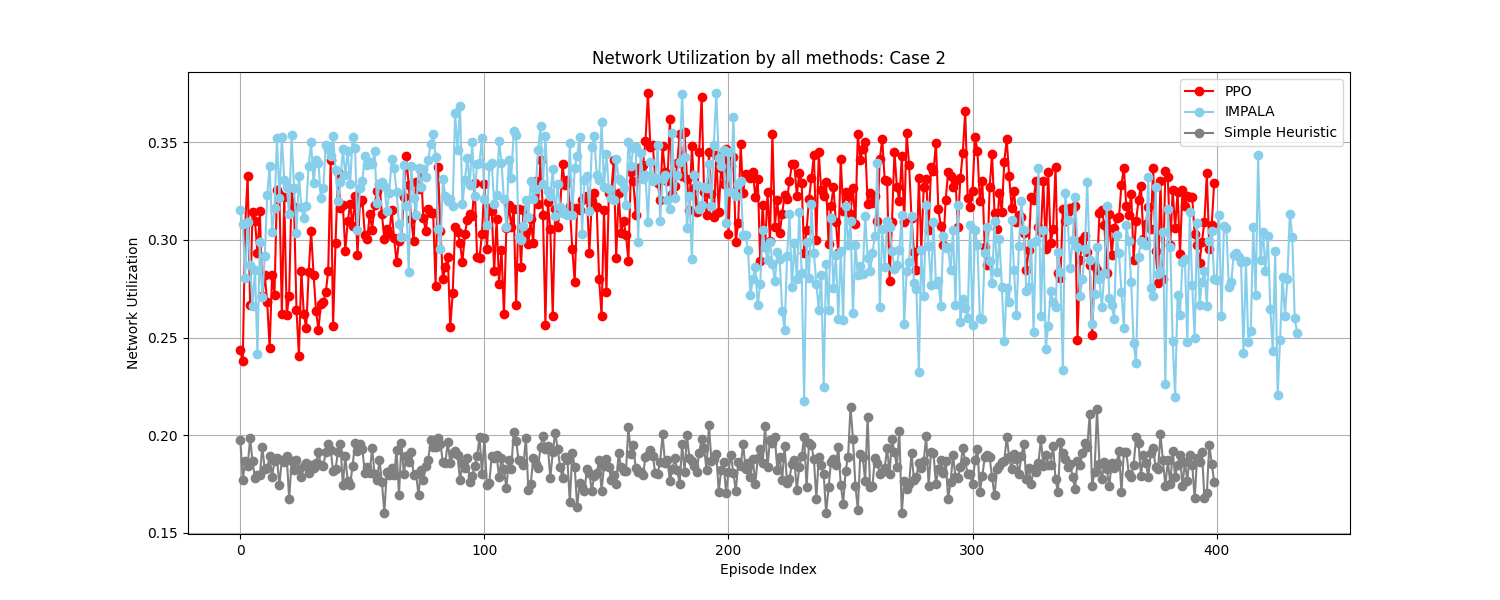
\includegraphics[width=\columnwidth]{images/comparison_case2.png}
    \caption{Comparison between methods for Case 2}
    \label{fig:comp_c2}
\end{figure}


\bibliography{ref}
\bibliographystyle{ieeetr}


\end{document}



